




\section{Aufgabenbeschreibung}
Beispielinhalt und Texte:
Das Thema der Seminararbeit gründet als Idee vor allem aus den folgenden beiden Beobachtungen aus privatem Lebensalltag und beruflicher Praxis: 
\begin{enumerate}
	\item Die seit den 2010er Jahren aufkommenden \textbf{smarten Technologien} finden im öffentlichen Raum und im Lebensalltag breiter Bevölkerungsschichten immer mehr Einzug. Drei Anwendungsbeispiele verdeutlichen und belegen das: 
	\begin{itemize}
	 \item Smart Watch: Uhren die z.B. um Fitness- und Nachrichtenfunktionen erweitert sind.
	 \item Smart TV: Fernsehgeräte die z.B. Zugriff auf Internet-Mediatheken erlauben.
	 \item Smart Home: Hausautomatisierungen und -steuerungen im privaten Bereich für  z.B. Licht und Heizung.
	 \end{itemize}

	 \item Das Aufkommen und der Erfolg der \textbf{PropTech\footnote{Kofferwort, englisch, aus 'property' (Immobilien) und 'technology' (Technologiegen)}-Branche} sowie die dieser Branche zuzuordnenden Unternehmen belegt die Relevanz von Innovation für die Wohnungswirtschaft ebenso wie die folgenden Erkenntnisse einer Studie \parencite[S. 18]{zia}:
	 \begin{itemize}
		 \item 72\% der befragten immobilienwirtschaftlichen Unternehmen nehmen Effizienzsteigerungen in Kernprozessen durch Einsatz digitaler Technologien an.
		 \item Weiter: Über ein Drittel gehen davon aus, dass Neugeschäft durch Einsatz digitaler Technologien generiert werden kann. 
	 \end{itemize}
\end{enumerate}

Vorgenannte Beobachtungen führen zu folgender Hypothese:

 \Rightarrow \textbf{Der Einsatz von smarten Displays in Quartieren der \ac{WoWi} ist möglich, wirtschaftlich und innovativ.}



\subsection{Was ist das Ziel der Projektarbeit?}
Beispielinhalt und Texte:
Als mögliche Standorte ergeben sich in Anlehnung an bisher übliche \glqq{}schwarze Bretter\grqq{} und \glqq{}Schaukästen\grqq{} in den Gebäuden sowie auch im Außenbereich vorhandenen Anlagen (Schaukästen, Werbeanlagen) auch für smarte Displays einige Vor- und Nachteile (Pro und Contra) die wie folgt stichpunktartig beschrieben werden: 

 \begin{itemize}
	 \item \textbf{Innenbereich:} 
	 \\ Wandmontage ebenso wie üblich und bekannte Schaukästen und schwarze Bretter im Windfang oder dem Etagenflur im Erdgeschoss eines Mietshauses.\\
	 \textbf{Pro:}\\
	  - Weiternutzung vorhandener, bewährter Montageorte \\
	  - Baurechtlich genehmigungsfrei \\
	  - Anbindung an Strom und Internet leichter als im Außenbereich \\
	  - Günstigere Bauart (kann weniger witterungsfest und vandalismussicher sein)\\
	 \textbf{Contra:}\\
	  - Wird wenig innovative Bauart zur Folge haben\\
	  - Kleinere Anzeigeflächen \\
	  - Nutzerkreis umfasst nur Mieter und Besucher des Hauses
	 \item \textbf{Außenbereich:} 
	 \\ Als freistehende Installation vor einem Wohngebäude, an einem markanten Wegepunkt im Quartier oder einem Innenhof eines Gebäudekomplexes.\\
	 \textbf{Pro:}\\
	  - Höhere Sichtbarkeit und Reichweite (nicht nur Mieter und Besucher eines Hauses, sondern auch Umfeld, Nachbarn und Durchgangsverkehr)  \\
	  - Attraktive Bauarten möglich \\
	  - Eröffnet weitergehende Nutzungsmöglichkeiten \\
	 \textbf{Contra:}\\
	  - Höhere Investitionskosten durch dem Standort geschuldete Bauart und Größe \\
	  - Erdarbeiten werden in der Regel nötig sein (Stromanschluss)  \\
	  - Baurechtlich genehmigungspflichtig, verursacht Mehrkosten und Aufwand
	  \item \textbf{Übergangsbereich Hauseingangstüre:} 
	  \\ Anbringung an Flächen die das Gebäude und den Außenbereich verbinden, beispielhaft genannt hier: Seitenteil der Türelemente im Hauseingangsbereich.\\
	  \textbf{Pro:}\\
	   - Unter Umständen umsetzbar als Modernisierungsmaßnahme (Nutzung als Videogegensprechanlage)  \\
	   - Technikaverse Bewohner und Besucher kommen zwangläufig in Kontakt mit dem smart Display \\
	  \textbf{Contra:}\\
	   -  Vorteile ergeben sich z.T. nur in noch nicht modernisiertem Bestand \\
	   -  Kleinerer Nutzerkreis und Anzeigefläche \\
 \end{itemize}

Eine weitergehende Bewertung oder Befürwortung einzelner Standorte soll hier nicht erfolgen um einzelne Anwendungsfälle nicht hier schon auszuschließen.


\subsection{Worin bestehen die (wahrscheinlichen) Herausforderungen? (allg. technisch und auch persönlich)}
Beispielinhalt und Texte:
Der Begriff soll daher hier geschärft werden um in der weiteren Verwendung un­miss­ver­ständ­lich zu sein.  

Die Definition erfolgt unter Bezug auf
\begin{enumerate}
	\item  die erfolgte Abgrenzung in 'enge' und 'weite' Definition nach \citeauthor{wirtschaftsfaktorimmo} (\citeyear[S. 9]{wirtschaftsfaktorimmo}) sowie
	\item die institutionelle Systematisierung der Immobilienwirtschaft nach \citeauthor{brauer2011einfuhrung} (\citeyear[S. 26]{brauer2011einfuhrung}).
\end{enumerate}

Die daraus entnommenen Zitate sollen hier im weiteren als gültige Definition für den verwendeten Begriff \textbf{Wohnungswirtschaft (WoWi)} gelten:  
\begin{itemize}
	\item Aus \citeauthor{wirtschaftsfaktorimmo} (\citeyear[S. 9]{wirtschaftsfaktorimmo}): \glqq{}alle Unternehmen, die an der Bewirtschaftung, Vermittlung und Verwaltung von Immobilien unmittelbar beteiligt sind\grqq{}. 
	 \item Sowie nach \citeauthor{brauer2011einfuhrung} (\citeyear[S. 36]{brauer2011einfuhrung}) zu den unterschiedlichen Rechtsformen \glqq{}(...)kommunalen, genossenschaftlichen und privaten Unternehmen(...)\grqq{} und den gleichwohl identischen Aufgabenfeldern: \glqq{}(...)nachhaltige Vermietung und Bestandsmanagement(...)\grqq{}.
\end{itemize}





\newpage
\section{Anforderungen}
Beispielinhalt und Texte:
Die genaue Zuordnung stellt sich also wie folgt dar:

\begin{table}[H]
	\caption{Zuordnung der Anforderungen der Hypothese zu den kritischen Anforderungen des Proof of Concept (PoC)}
	\label{tbl:zuordnungHypothesePoc}
	\begin{tabularx}{\textwidth}[ht]{|l|c|X|}
	\hline
	\textbf{Anforderung der Hypothese} & \textbf{Zuordnung} & \textbf{Abbildung in \ac{PoC}} \\
	\hline\hline 
	ist möglich & \Leftrightarrow & Prüfung der Machbarkeit  \\
	\hline 
	ist wirtschaftlich & \Leftrightarrow &  Effizienz-Faktoren aufzeigen \\
	\hline 
	ist innovativ & \Leftrightarrow &  Nutzbarkeit und Anwendungsfälle \\
	\hline
	\end{tabularx}
\end{table}


\subsection{Welche Techniken/ Technologien sollen eingesetzt werden, um die Aufgabe zu lösen/ realisieren?}
Beispielinhalt und Texte:

Eine Betrachtung der Wirtschaftlichkeit einer Einzelinvestition in ein smart Display in einem Quartier könnte damit nach z.B. folgendem Schema erfolgen:


\begin{table}[H]
	\caption{Mögliches Schema einer Wirtschaftlichkeits- und Effizienzbetrachtung der Einzelinvestition in smart Displays}
	\label{tbl:SchemaWBsmartDisplay}
	\begin{tabularx}{\textwidth}[ht]{cl}
	\hline
	\textbf{ - }   &  Investitionskosten (der Einzelmaßnahme) \\
	\textbf{ - }   &  lfd. Betriebs- und Wartungskosten  \\
	\textbf{ + }   &  lfd. Einsparung Personalkosten  \\
	\textbf{ + }   &  Refinanzierung als Modernisierungsmaßnahme   \\
	\textbf{ + }   &  Umlage von (Teilen der) Betriebskosten auf Gebäudenutzer  \\
	\textbf{ + }   &  Mehrerlöse durch Überlassung als Werbefläche an Dritte  \\
	\hline\hline
	\textbf{ = }   &  \textbf{in Euro messbare Wirtschaftlichkeit} \\
	\textbf{ + }   &  Digitalisierung eines Geschäftsprozesses  \\
	\textbf{ + }   &  Imagegewinn für das Quartier \\
	\textbf{ + }   &  Öffentlichkeitswirksame Einführung und Realisierung  \\
	\hline\hline
	\textbf{ = }   &  \textbf{gesamt zu bewertende Effizienz} \\
	\hline
\end{tabularx}
\end{table}

Kommt man nun zurück auf die Definition des Bergriffs der Effizienz nach \citeauthor{eichhorn2016} (\citeyear[S. 183 f.]{eichhorn2016}), kann man feststellen, dass es für die Beurteilung wesentliche Faktoren gibt, die nicht der Wirtschaftlichkeit zuzurechnen sind.



\subsection{Warum sollen gerade diese eingesetzt werden?}
Beispielinhalt und Texte:
Mit smarten Displays sind in dieser Seminararbeit nicht die von Desktop-Computer abnehmbaren und tragbaren LCD-Monitore gemeint die 2002 im Zusammenhang mit Microsofts Betriebssystem \glqq{}Windows CE for Smart Displays\grqq{} vorgestellt wurden \parencite{heise-ms-sd} und im Jahr 2004 wieder eingestellt worden sind \parencite{ct-3-2004}. 

\begin{figure}[H]
	\caption{Handteil eines smart Displays nach Microsoft-Konzept}\label{fig:HandteilMSsmartDisplay}
	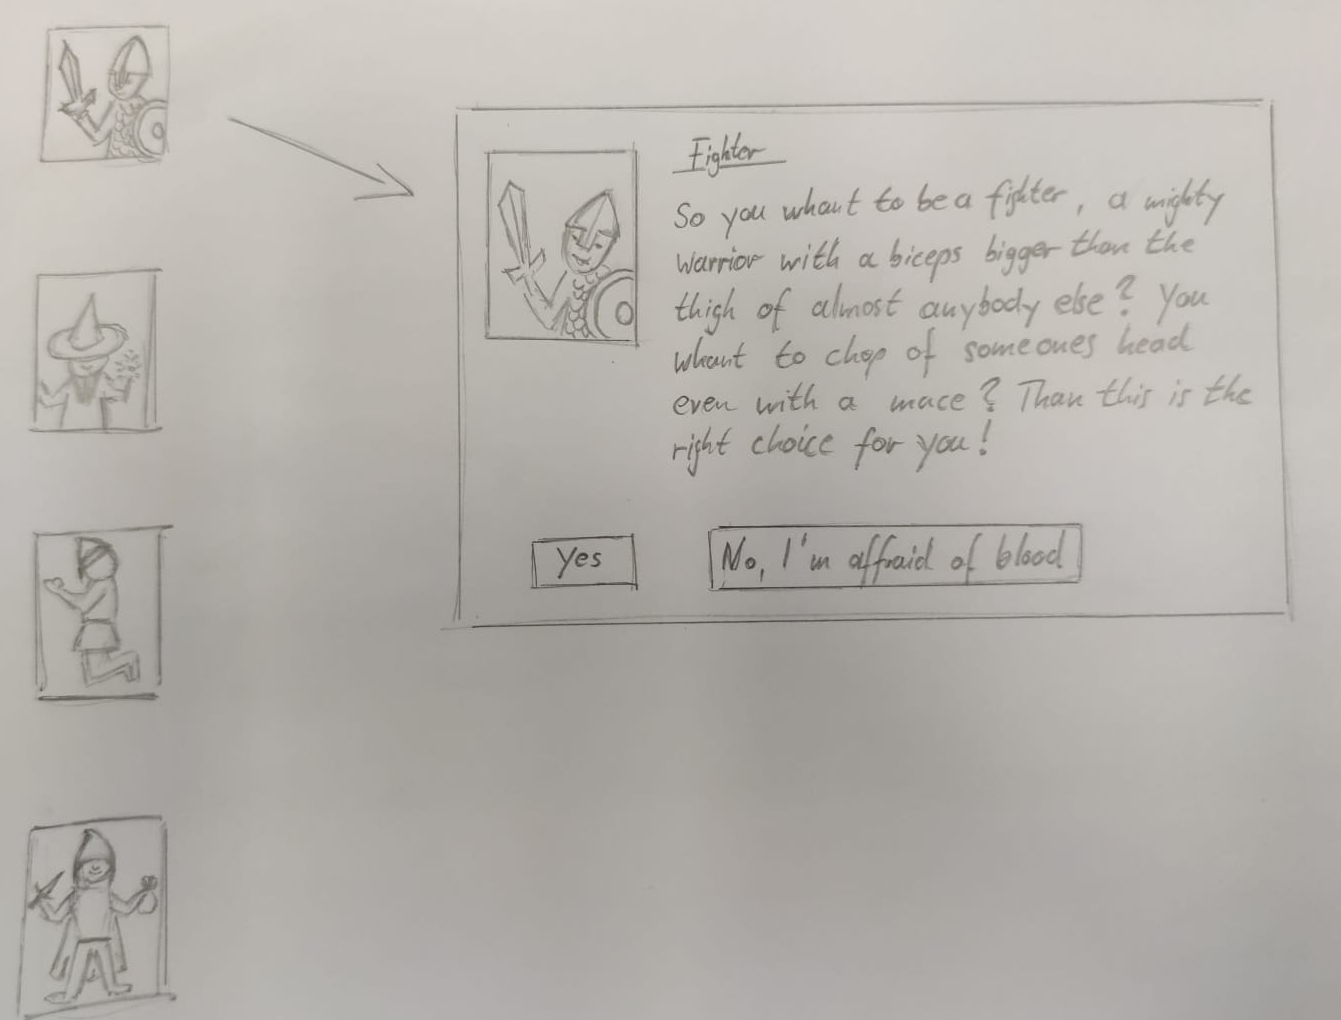
\includegraphics[height=5cm,keepaspectratio]{2021-11-29-Entwurf-Klassen-Ui}
	\\
	Quelle: Homepage von Mark Strehlow, Senior Interaction Designer\\ im Projekt Mira (\href{https://msdo.us/Microsoft-Mira}{msdo.us/Microsoft-Mira})
\end{figure}

Vielmehr sind hier erst noch durch Forschung und Entwicklung für die \ac{WoWi} zu schaffenden und nutzbar zu machenden Geräte gemeint.


\subsection{Gibt es besondere Anforderungen? (technisch, Benutzer, sonstige)}
Beispielinhalt und Texte:

\newpage
\section{Herangehensweise}
Beispielinhalt und Texte:

\subsection{Wie soll das Ziel erreicht werden (Vorgehen, Architektur)}
Beispielinhalt und Texte:

\newpage
\section{Vorstellung des Ergebnisses}
Beispielinhalt und Texte:

\newpage
\section{Reflektion}
Beispielinhalt und Texte:

 die Anwendung wird hier durch eine Betrachtung  der untenstehenden Punkte erfolgen: 
\begin{itemize}
	\item \textbf{Prüfung rechtlicher und IT-technischer Machbarkeit:}
	\\ Neben baurechtlicher Betrachtung hier auch Prüfung in Bezug auf verschiedenartige Realisierungen in Größe, Standort, Bauart und IT-Integration.
	\item \textbf{Aufzeigen und erörtern relevanter Effizienz-Faktoren:}
	\\ Umfasst typisch erwartbare Effizienz-Faktoren wie die Wirtschaftlichkeit ebenso wie auch darüber hinausgehende Auswirkungen die zur ebenso zur Effizienz zu zählen sind.
	\item \textbf{Darstellung möglicher Nutzbarkeiten und Anwendungsfälle:}
	\\ Ausführungen zu erwartbaren Einflüssen auf vorhandene Geschäftsprozesse in der \ac{WoWi} aber auch durch Aufzeigen von neuartigen und darüber hinausgehenden Anwendungsfällen und -bereichen.
\end{itemize}

Diese drei vorgenannten Punkte spiegeln die drei Anforderungen aus der Hypothese der Einleitung wieder und entsprechen dieser genau, in den jeweils genannten Reihenfolgen. 


